\documentclass{article}\usepackage[]{graphicx}\usepackage[]{color}
%% maxwidth is the original width if it is less than linewidth
%% otherwise use linewidth (to make sure the graphics do not exceed the margin)
\makeatletter
\def\maxwidth{ %
  \ifdim\Gin@nat@width>\linewidth
    \linewidth
  \else
    \Gin@nat@width
  \fi
}
\makeatother

\definecolor{fgcolor}{rgb}{0.345, 0.345, 0.345}
\newcommand{\hlnum}[1]{\textcolor[rgb]{0.686,0.059,0.569}{#1}}%
\newcommand{\hlstr}[1]{\textcolor[rgb]{0.192,0.494,0.8}{#1}}%
\newcommand{\hlcom}[1]{\textcolor[rgb]{0.678,0.584,0.686}{\textit{#1}}}%
\newcommand{\hlopt}[1]{\textcolor[rgb]{0,0,0}{#1}}%
\newcommand{\hlstd}[1]{\textcolor[rgb]{0.345,0.345,0.345}{#1}}%
\newcommand{\hlkwa}[1]{\textcolor[rgb]{0.161,0.373,0.58}{\textbf{#1}}}%
\newcommand{\hlkwb}[1]{\textcolor[rgb]{0.69,0.353,0.396}{#1}}%
\newcommand{\hlkwc}[1]{\textcolor[rgb]{0.333,0.667,0.333}{#1}}%
\newcommand{\hlkwd}[1]{\textcolor[rgb]{0.737,0.353,0.396}{\textbf{#1}}}%
\let\hlipl\hlkwb

\usepackage{framed}
\makeatletter
\newenvironment{kframe}{%
 \def\at@end@of@kframe{}%
 \ifinner\ifhmode%
  \def\at@end@of@kframe{\end{minipage}}%
  \begin{minipage}{\columnwidth}%
 \fi\fi%
 \def\FrameCommand##1{\hskip\@totalleftmargin \hskip-\fboxsep
 \colorbox{shadecolor}{##1}\hskip-\fboxsep
     % There is no \\@totalrightmargin, so:
     \hskip-\linewidth \hskip-\@totalleftmargin \hskip\columnwidth}%
 \MakeFramed {\advance\hsize-\width
   \@totalleftmargin\z@ \linewidth\hsize
   \@setminipage}}%
 {\par\unskip\endMakeFramed%
 \at@end@of@kframe}
\makeatother

\definecolor{shadecolor}{rgb}{.97, .97, .97}
\definecolor{messagecolor}{rgb}{0, 0, 0}
\definecolor{warningcolor}{rgb}{1, 0, 1}
\definecolor{errorcolor}{rgb}{1, 0, 0}
\newenvironment{knitrout}{}{} % an empty environment to be redefined in TeX

\usepackage{alltt}
\title{Descriptive Analyses} 
\author{Francois Rerolle}
\date{\today}

%List if latex packages you'll need
\usepackage{float}
\usepackage{mathtools}
\usepackage{graphicx}
\graphicspath{{/Users/francoisrerolle/Desktop/UCSF/Dissertation/Paper-1-Geospatial-Analysis-Forest-Incidence/Analyses/Descriptive_Analyses/figure/}}

%set the margins of the document
\usepackage[]{geometry}

%End the preamble and begin the document
\IfFileExists{upquote.sty}{\usepackage{upquote}}{}
\begin{document}
\maketitle
 

\noindent \textit{Report of some descriptive statistics on the final cleaned dataset (A3 + environmental covariates).}

%%%%%%%%%%%%%%%%%%%%%%%%%%%%%%%%%%%%%%%%%
% Start by a description of the dataset %
%%%%%%%%%%%%%%%%%%%%%%%%%%%%%%%%%%%%%%%%%

\section{Description of dataset}
\subsection{What, where and when}
In 2017, we collected all A3 forms available in 4 districts of the southern province of Champasak in Laos: Moonlapamok, Pathoomphone, Sanasomboon and Sukhuma. A3 forms record all suspected malaria cases passively detected that got tested for malaria by RDT and/or microscopy.\\

\noindent A total of \(64501\) A3 forms were collected. Individuals reported coming from \(505\) villages (\(4.2\) $\%$ missing) in \(7\) districts (\(0\) $\%$ missing). Most individuals lived in districts where A3 form was collected but some lived in other districts:\\

\begin{knitrout}
\definecolor{shadecolor}{rgb}{0.969, 0.969, 0.969}\color{fgcolor}\begin{kframe}
\begin{verbatim}
## 
##    Champasak        Khong  Moonlapamok     Paksxong Pathoomphone 
##          958          578        15741            2        24316 
##   Phongthong  Sanasomboon      Sukhuma         <NA> 
##            3        14158         8747            0
\end{verbatim}
\end{kframe}
\end{knitrout}

\noindent Figure \ref{fig:Histogram_Date} shows a time distribution of A3 forms ranging from \(2013-09-25\) to \(2016-12-29\), pretty constant over a 3 year period from October 2013 to October 2016. Figure \ref{fig:Histogram_Date_District} shows that this true across the 4 districts of data collection.

\begin{figure}
\begin{center}

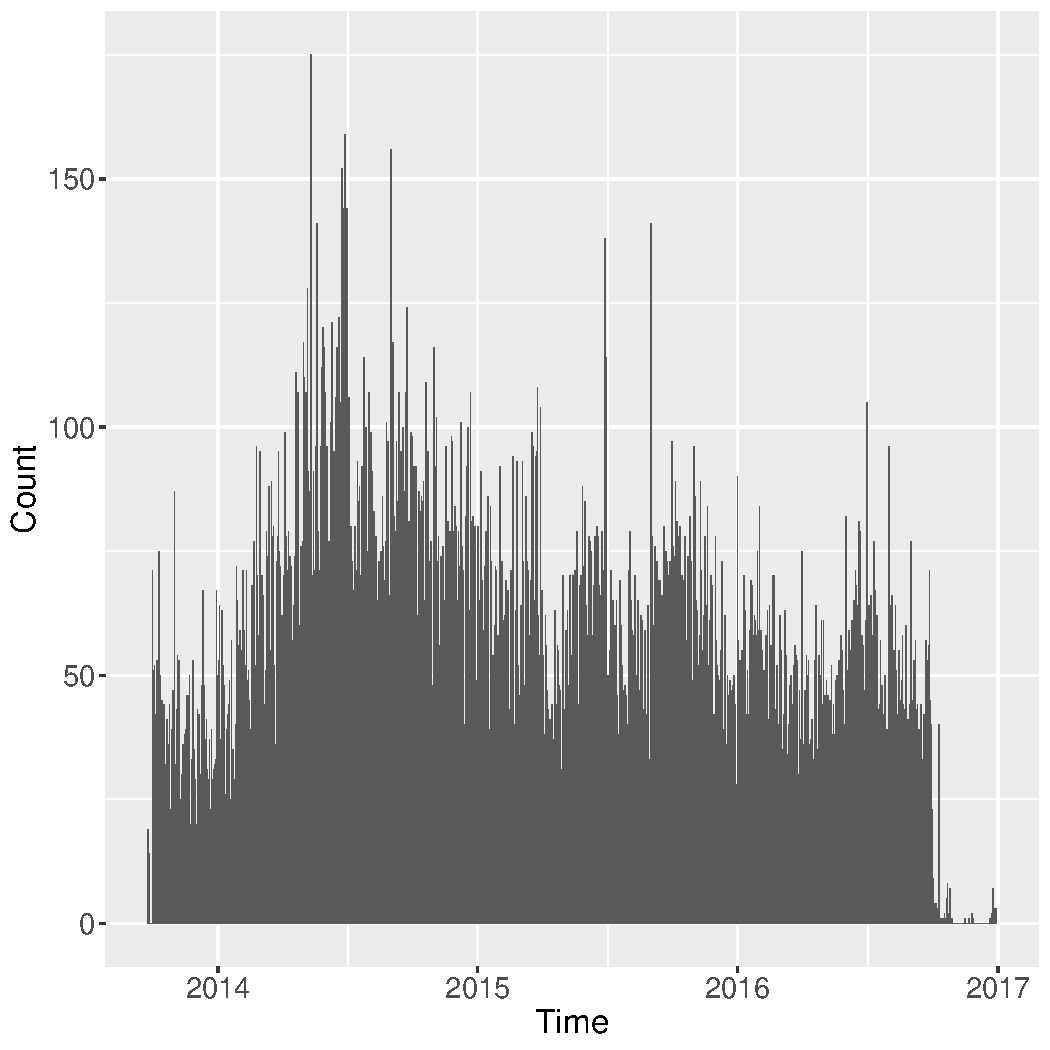
\includegraphics[width=0.5\textwidth]{fig1-1}
\end{center}
\caption{Histogram of A3 data collection times.}
\label{fig:Histogram_Date}
\end{figure}

\begin{figure}
\begin{center}

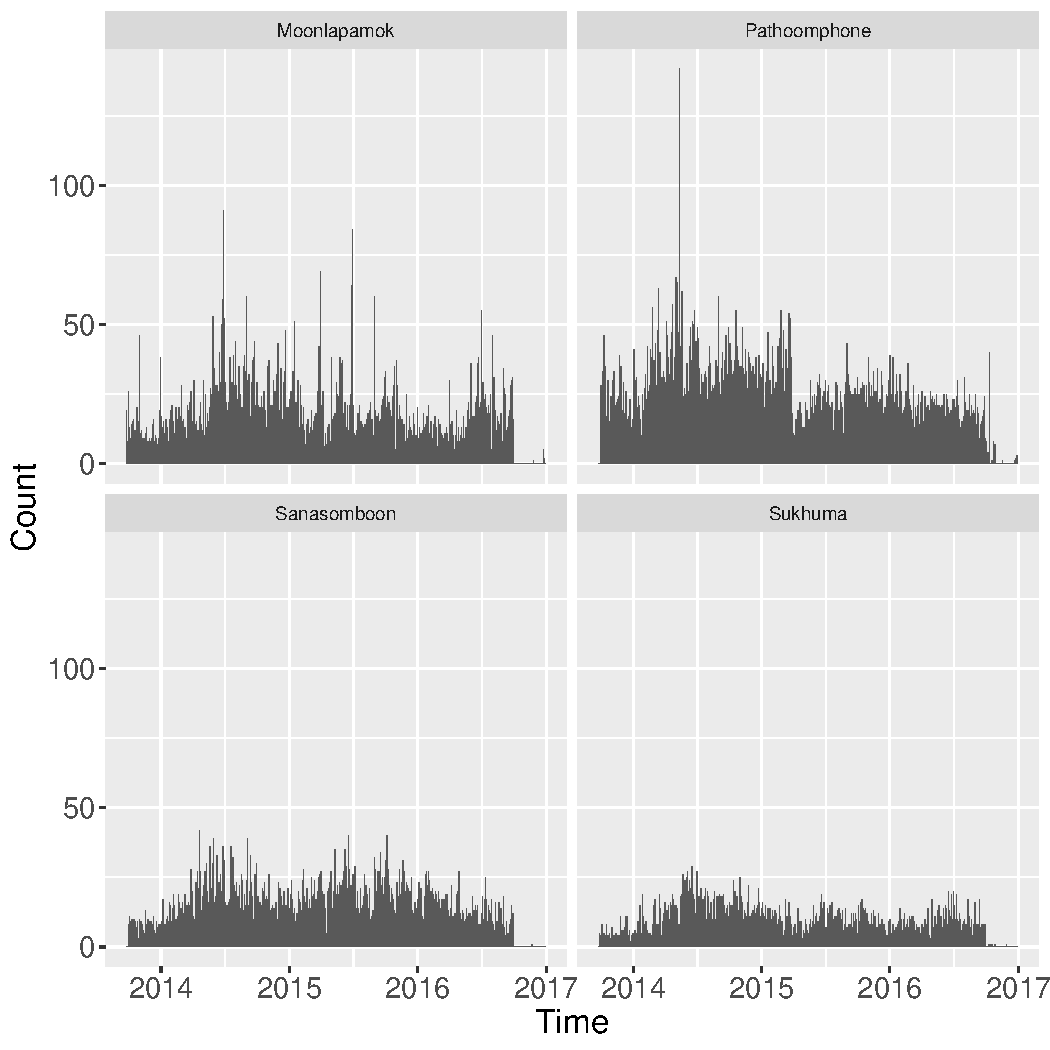
\includegraphics[width=0.5\textwidth]{fig2-1}
\end{center}
\caption{Histogram of A3 data collection times per district.}
\label{fig:Histogram_Date_District}
\end{figure}

\subsection{Description of variables}
There are two types of variables available in this dataset:
\begin{itemize}
\item Variables that were collected in the A3 form: date, district, village, age, gender, occupation, RDT result, microscopy result and treatment taken.
\item Environmental covariates that were extracted from raster layers via GPS coordinates of villages (matched via offical list of villages in Champasak): altitude, temperature, precipitation, population, forest percent in 1km and 10km for the data collection and previous 5 years.
\end{itemize}

%%%%%%%%%%%%%%%%%%%%%%%%%%
% Descriptive Statistics %
%%%%%%%%%%%%%%%%%%%%%%%%%%

\section{Descriptive statistics}
\subsection{Basic description}
\subsubsection{A3 variables} 

% Table for A3 variables

\begin{table}[htp]
\begin{center}
\begin{tabular}{lp{10.5cm}c}
Variable & Description & Missing \\ \hline
&& \\
Date & Date of the A3 interview, over 3 years from October 2013 to 2016. & \(0.3\) $\%$ \\
&& \\
District & Reported district where living. \(8\) different districts of Champasak Province. \(97.6\) $\%$ come from the 4 districts where A3 forms where collected: MP, PT, SB and SK. & \(0\) $\%$ \\
&& \\
Village & Reported village where living. \(506\) different villages of Champasak Province, \(497\) in MP, PT, SB or SK. & \(4.2\) $\%$ \\ 
&& \\
Age & Reported age. Ranges from \(0\) to \(98\), with a median of \(26\) years. & \(0.7\) $\%$ \\ 
&& \\
Male & Reported gender. \(71\) $\%$ of males. & \(2.2\) $\%$ \\ 
&& \\
Occupation & Reported occupation. \(6\) different occupations. \(67.7\) $\%$ are farmers. & \(8.7\) $\%$ \\ 
&& \\ \hline
&& \\
RDT & RDT results. \(16.9\) $\%$ Pf, \(19.4\) $\%$ Pv and \(1.8\) $\%$ mix. & \(29.4\) $\%$ \\ 
&& \\
Microscopy & Microscopy results. \(8\) $\%$ Pf, \(10.7\) $\%$ Pv and \(1.7\) $\%$ mix. & \(75.7\) $\%$ \\ 
&& \\
Treatment & Treatment provided to A3 individuals. \(4\) different treatment combinations. \(78\) $\%$ received no treatment and \(21.3\) $\%$ received Coartem alone. & \(0.1\) $\%$ \\ 
&& \\ \hline
&& \\
GPS & GPS coordinates of villages matched with official list of villages in Champasak with GPS. Environmental covariates were extracted for all villages with GPS coordinates. & \(11.1\) $\%$ \\ 
&& \\ \hline

\end{tabular}
\caption{Basic description of A3 variables in dataset.}
\label{table:Table_Basic_Description_A3}
\end{center}
\end{table}

\newpage

\subsubsection{Environmental variables}

% Table for environmental variables

\begin{table}[htp]
\begin{center}
\begin{tabular}{lp{10.5cm}c}
Variable & Description & Missing \\ \hline
&& \\
Altitude & Altitude, extracted from SRTM with resolution 1km. Ranges from  \(89\) to \(301\), with a mean of \(128\) and a median of \(114\) meters. & \(11.4\) $\%$ \\
&& \\
Temperature & Mean annual temperature, extracted from worldclim with resolution 1km. Ranges from  \(25.6\) to \(27\), with a mean of \(27\) and a a median of \(26.8\) $^\circ$C. We also have a measure of seasonality with the standard deviation. & \(11.1\) $\%$ \\
&& \\
Precipitation & Total annual precipitation, extracted from worldclim with resolution 1km. Ranges from  \(1831\) to \(2550\), with a mean of \(2193\) and a a median of \(2193\) millimeters. We also have a measure of seasonality with the coefficient of variation. & \(11.1\) $\%$ \\
&& \\
Population & Population, extracted from worldpop with resolution 100m, aggregated at 1km. Ranges from  \(9\) to \(402\), with a mean of \(61\) and a median of \(52\) habitants in $km^{2}$. Available for 2010 and 2015. & \(11.1\) $\%$ \\
&& \\ \hline
&& \\
Forest & Percent forest within 10 km (\textit{resp.} 1 km), computed from landcover (High-Biomass Vegetation) layers produced via classification algorithm on remote landsat data. Ranges from  \(0\) to \(83.1\) (\textit{resp.} \(0\) to \(97.8\)), with a mean of \(27.3\) $\%$ (\textit{resp.} \(5.9\)) and a median of \(25.1\) $\%$ (\textit{resp.} \(0.4\)). & \(11.5\) $\%$ \\
&& \\
Forest change & Absolute percent forest change within 10 km (\textit{resp.} 1 km), in previous 2 years. Ranges from  \(-11.4\) to \(8.4\) (\textit{resp.}  \(-32.2\) to \(32.7\)), with a mean of \(-2.7\) $\%$ (\textit{resp.} \(-1.8\)) and a median of \(-3\) $\%$ (\textit{resp.} \(-0.2\)). Available for previous 5 years. & \(11.5\) $\%$ \\
&& \\ \hline

\end{tabular}
\caption{Basic description of environmental variables in dataset.}
\label{table:Table_Basic_Description_Environmental}
\end{center}
\end{table}

\newpage

\subsection{Descriptive summary}
\subsubsection{A3 variables}

% A3 variables pie charts

\begin{figure}[hbp]
\begin{center}

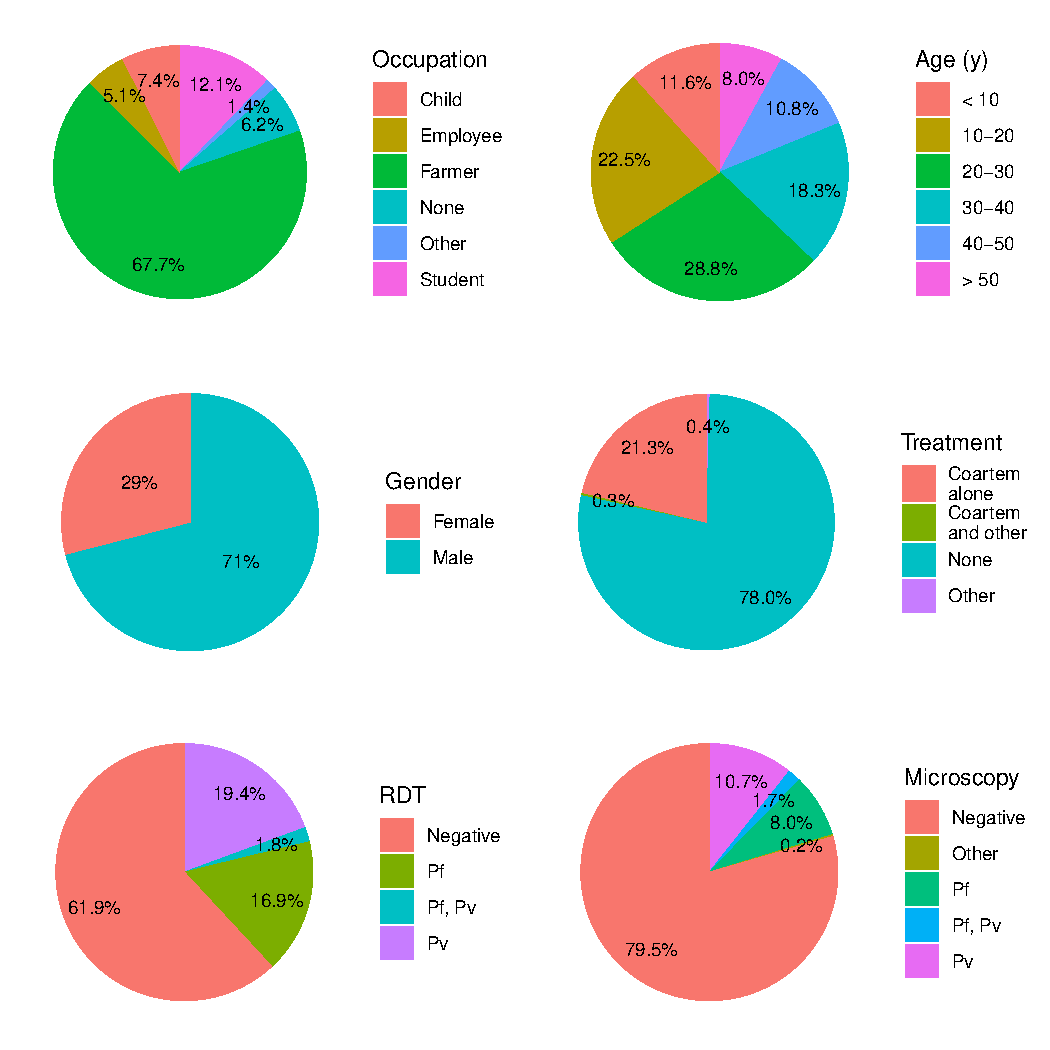
\includegraphics[width=0.9\textwidth]{fig3-1}
\end{center}
\caption{Pie charts of A3 variables.}
\label{fig:Pie_Chart_A3}
\end{figure}

\newpage
\subsubsection{Environmental variables}
% Environmental variables histograms

\begin{figure}[hbp]
\begin{center}

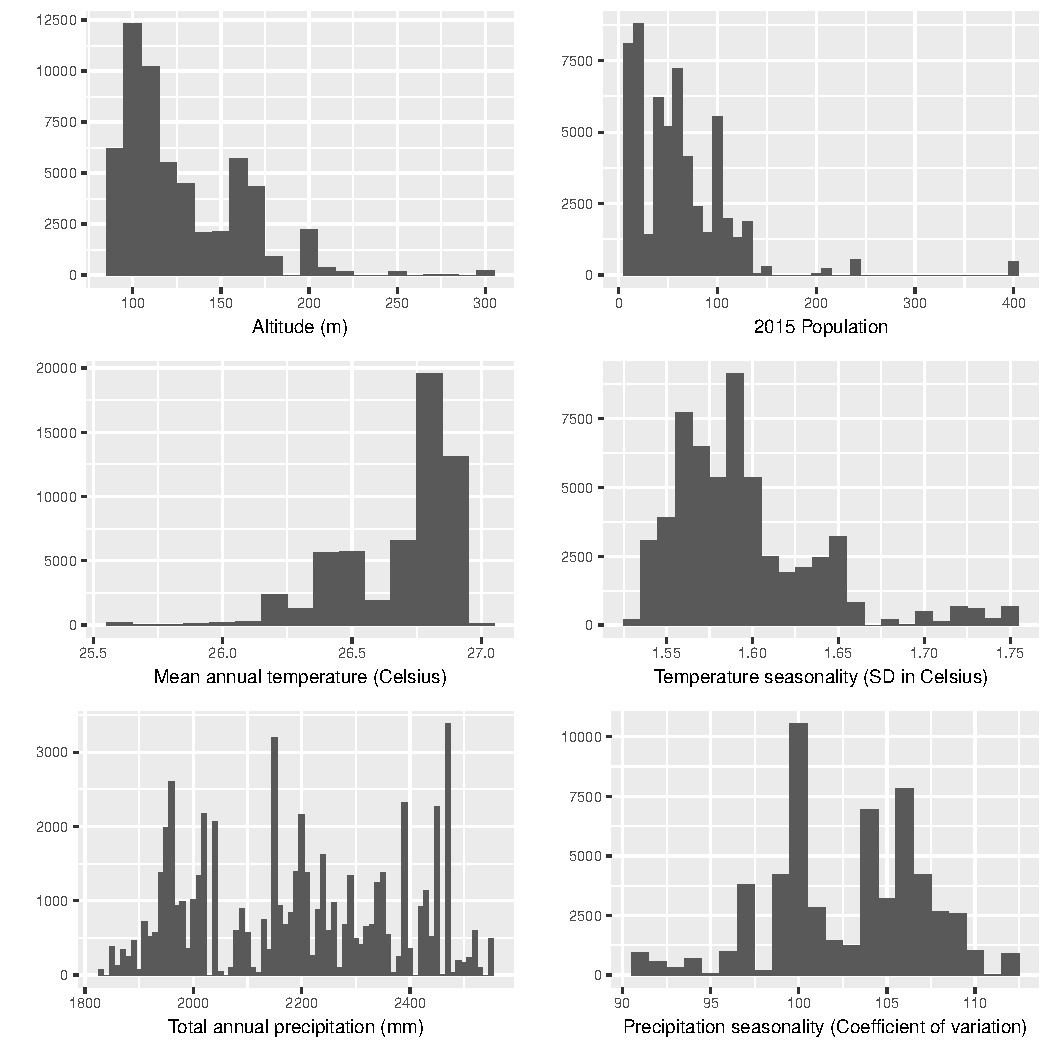
\includegraphics[width=0.9\textwidth]{fig4-1}
\end{center}
\caption{Histogram of environmental covariates at A3 villages.}
\label{fig:Histogram_Environmental_Covariates}
\end{figure}

\newpage
\subsubsection{Forest variables}
% Forest variables histograms

\begin{figure}[hbp]
\begin{center}

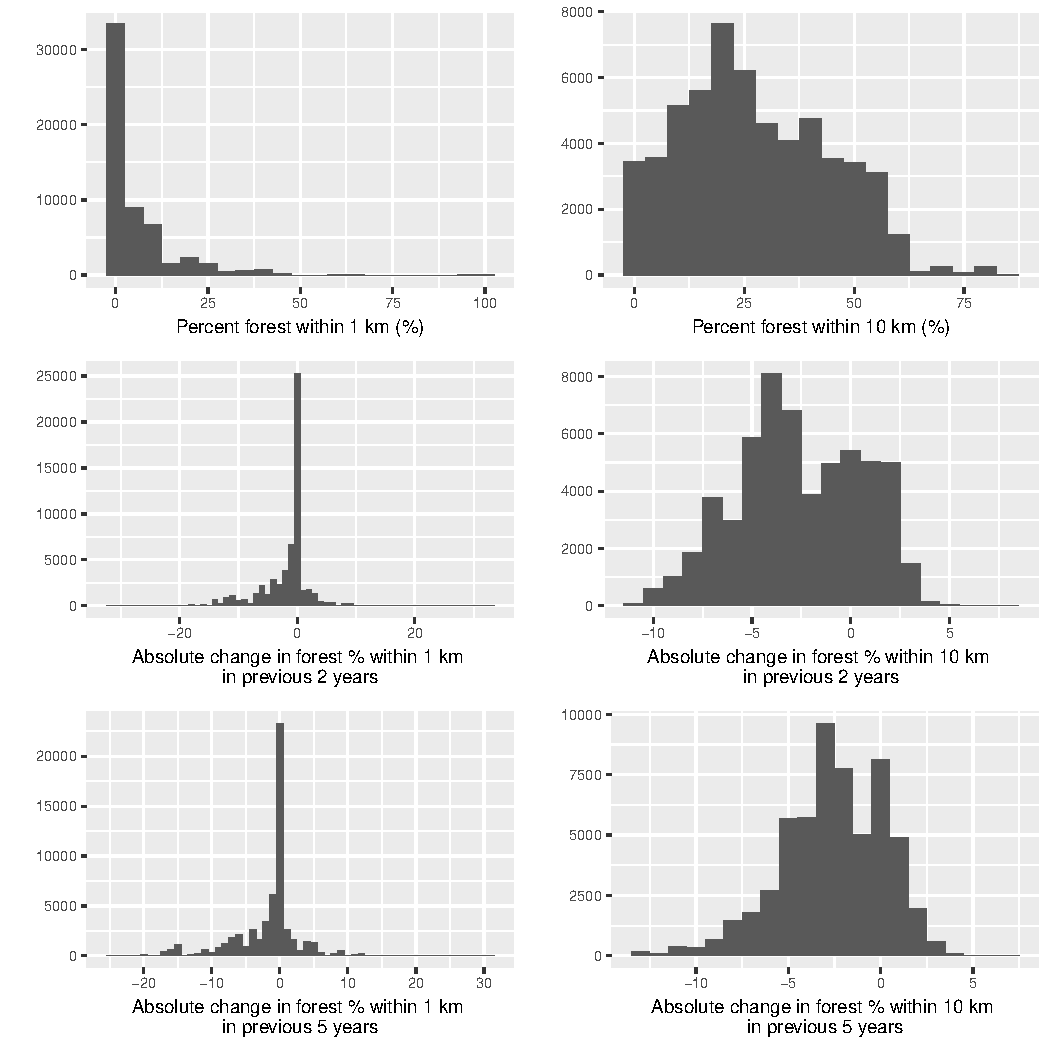
\includegraphics[width=0.9\textwidth]{fig5-1}
\end{center}
\caption{Histogram of forest covariates at A3 villages.}
\label{fig:Histogram_Forest_Covariates}
\end{figure}

\newpage

\subsection{Variables' correlations}

\begin{figure}[hbp]
\begin{center}
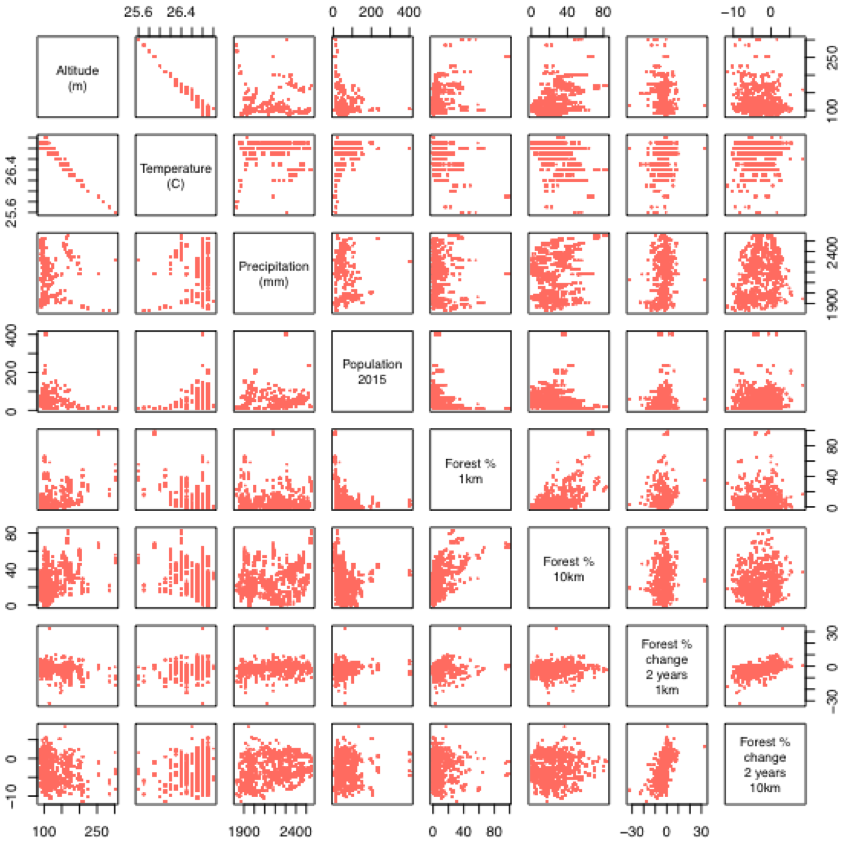
\includegraphics[width=0.9\textwidth]{fig6-manual}
\end{center}
\caption{Correlogram of variables in dataset.}
\label{fig:Correlogram_Covariates}
\end{figure}

\newpage
\subsection{Unadjusted associations between forest and malaria}
\subsubsection{Plasmodium Falciparum}

%%%%%%%%%%% PF

\begin{figure}[hbp]
\begin{center}

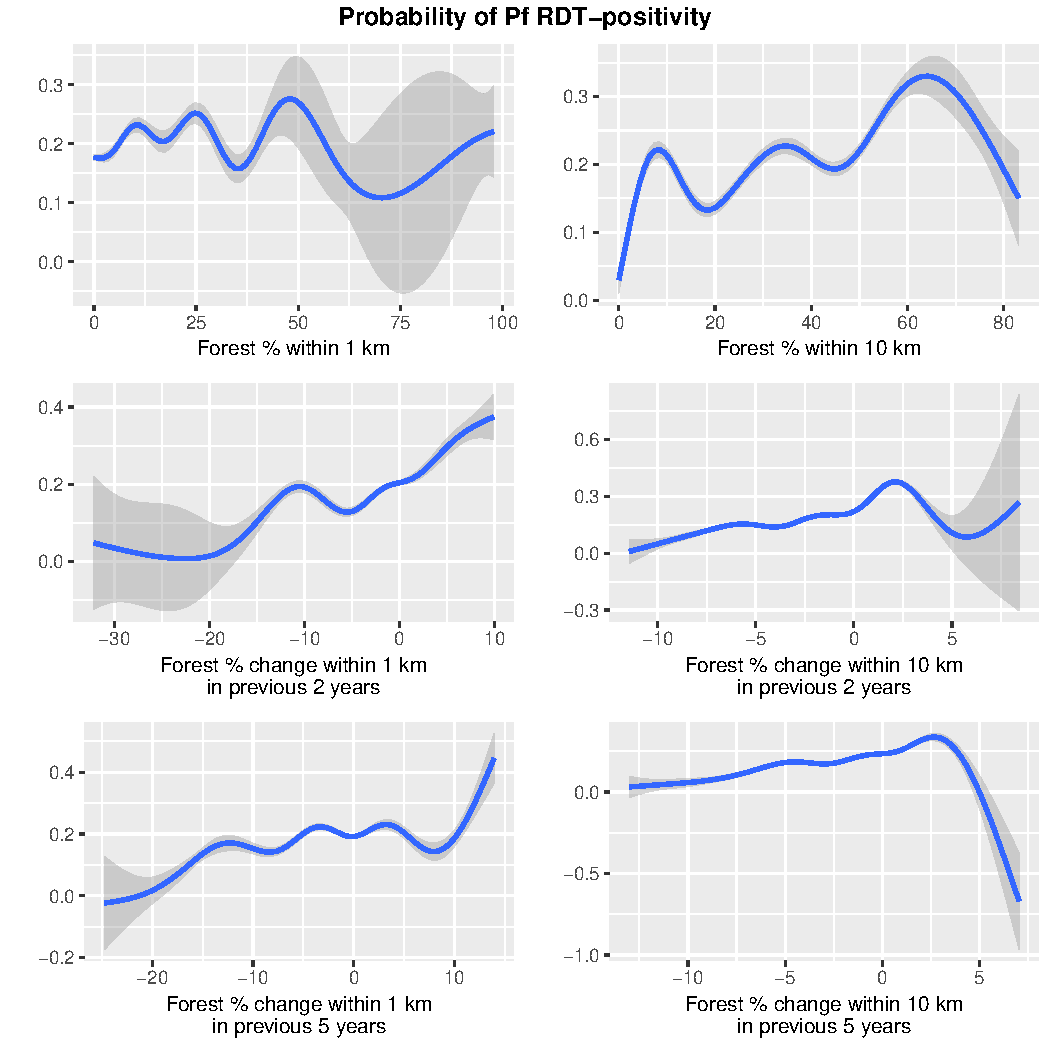
\includegraphics[width=0.9\textwidth]{fig7-1}
\end{center}
\caption{GAM smooth plots of association between forest and Pf RDT positivity.}
\label{fig:Smooth_Pf_RDT}
\end{figure}


\begin{figure}[hbp]
\begin{center}

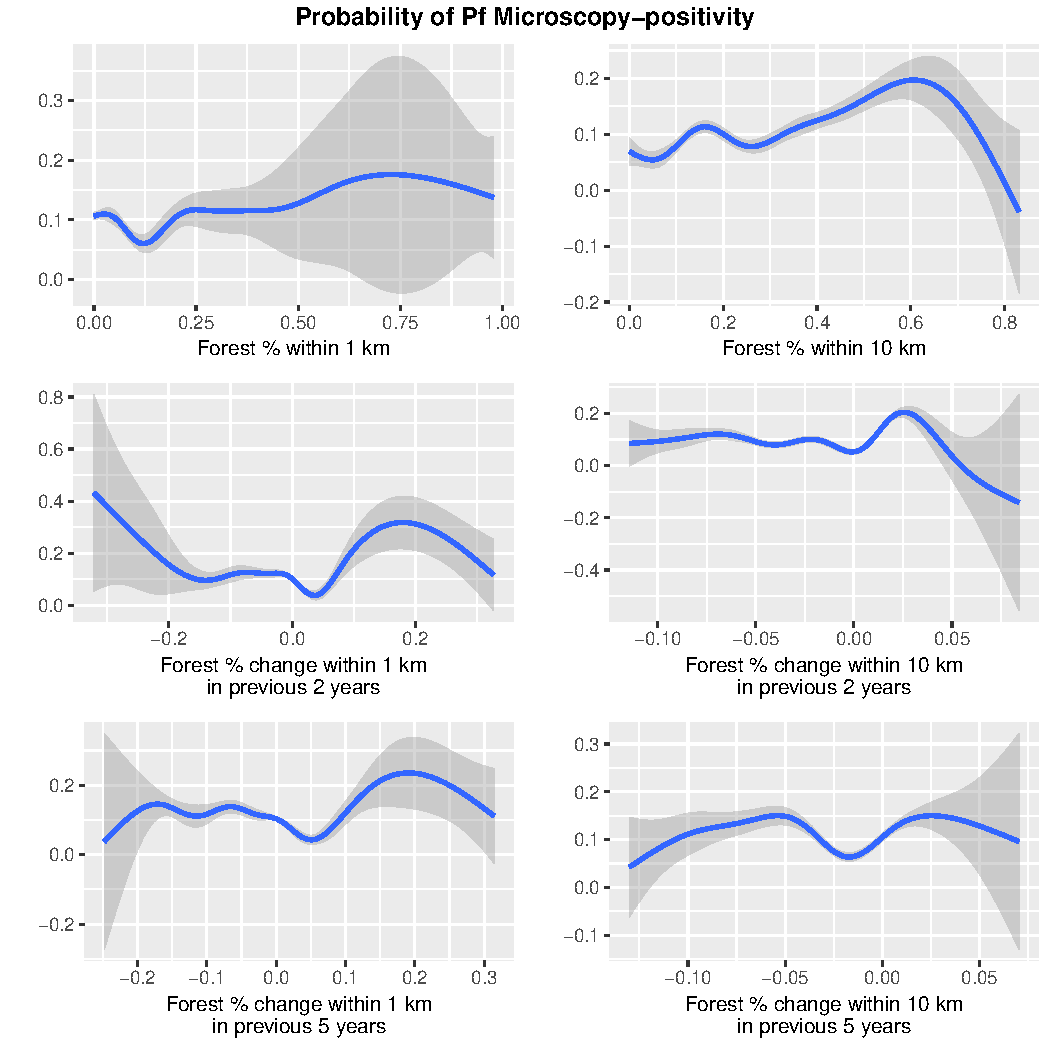
\includegraphics[width=0.9\textwidth]{fig8-1}
\end{center}
\caption{GAM smooth plots of association between forest and Pf Microscopy positivity.}
\label{fig:Smooth_Pf_Microscopy}
\end{figure}

\newpage

\subsubsection{Plasmodium Vivax}

%%%%%%%%%%% PV

\begin{figure}[hbp]
\begin{center}

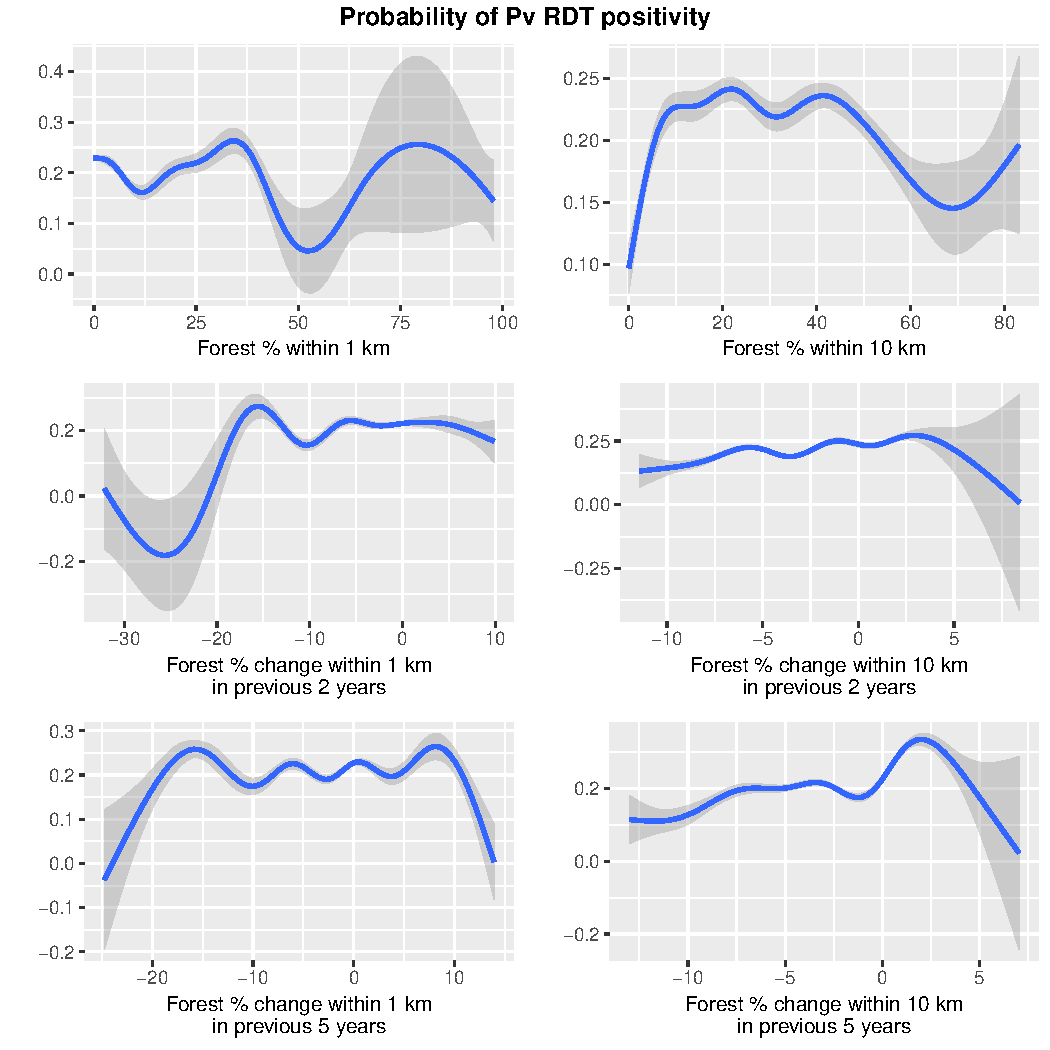
\includegraphics[width=0.9\textwidth]{fig9-1}
\end{center}
\caption{GAM smooth plots of association between forest and Pv RDT-positivity.}
\label{fig:Smooth_Pv_RDT}
\end{figure}


\begin{figure}[hbp]
\begin{center}

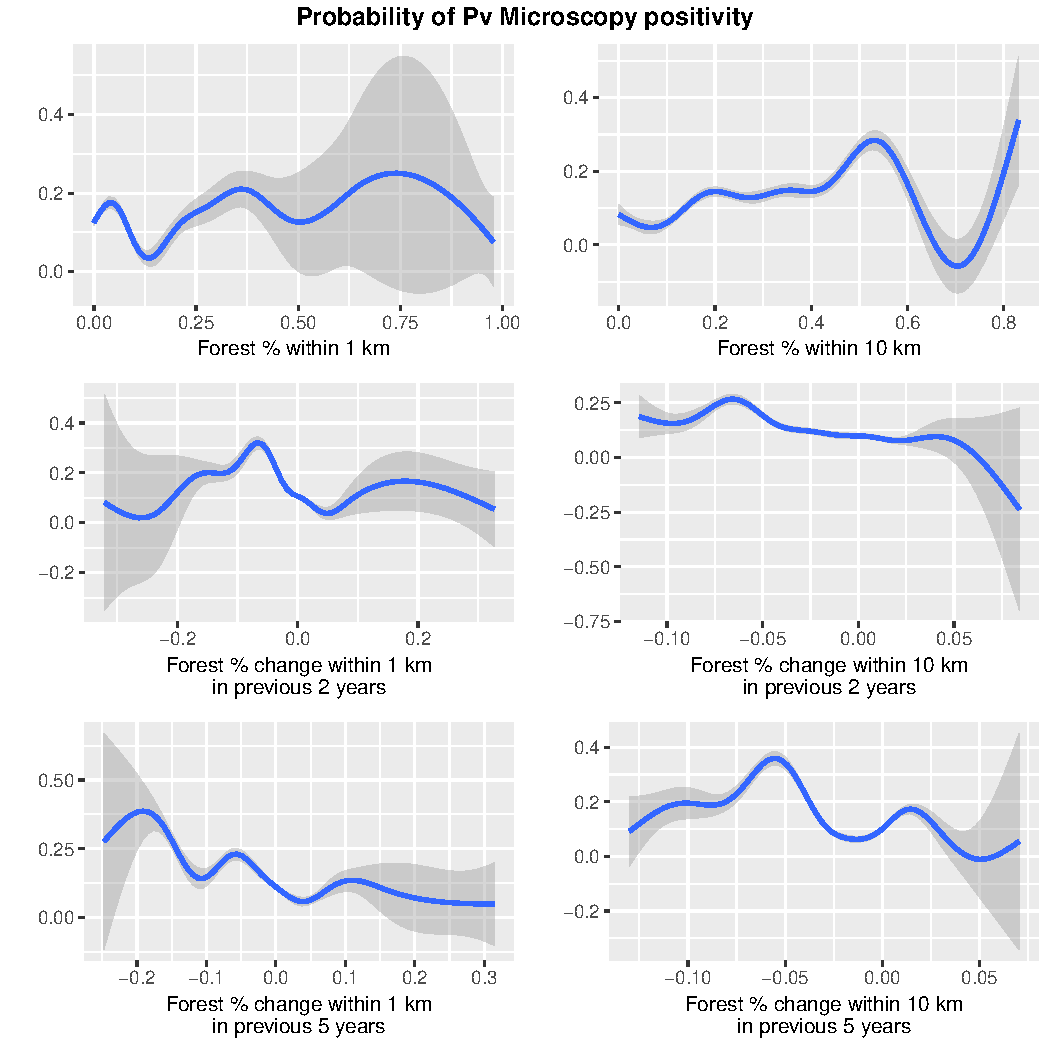
\includegraphics[width=0.9\textwidth]{fig10-1}
\end{center}
\caption{GAM smooth plots of association between forest and Pv Microscopy positivity.}
\label{fig:Smooth_Pv_Microscopy}
\end{figure}

\end{document}
